
\documentclass{acmsiggraph}               % final
%\documentclass[review]{acmsiggraph}      % review
%\documentclass[widereview]{acmsiggraph}  % wide-spaced review
%\documentclass[preprint]{acmsiggraph}    % preprint

%% Uncomment one of the four lines above depending on where your paper is
%% in the conference process. ``review'' and ``widereview'' are for review
%% submission, ``preprint'' is for pre-publication, and ``final'' is for
%% the version to be printed.

%% These two line bring in essential packages: ``mathptmx'' for Type 1
%% typefaces, and ``graphicx'' for inclusion of EPS figures.

\usepackage{mathptmx}
\usepackage{graphicx}
\usepackage{epsfig}
\usepackage{amsmath,amscd,amssymb}

\newtheorem{theorem}{Theorem}[section]
\newtheorem{proposition}[theorem]{Proposition}
\newtheorem{definition}[theorem]{Definition}
\newtheorem{lemma}[theorem]{Lemma}
\newtheorem{corollary}[theorem]{Corollary}
\newtheorem{remark}[theorem]{Remark}


%% use this for zero \parindent and non-zero \parskip, intelligently.

\usepackage{parskip}

%% If you are submitting a paper to the annual conference, please replace
%% the value ``0'' below with your OnlineID. If you are not submitting this
%% paper to the annual conference, you may safely leave it at ``0'' -- it
%% will not be included in the output.

\onlineid{0}

%% need to document this!

\acmformat{cameraready}

%% Paper title.

\title{Cartoon-Looking Rendering of 3D-Scenes Implementation}

%% Author and Affiliation (single author).

%%\author{Roy G. Biv\thanks{e-mail: roy.g.biv@aol.com}\\Allied Widgets Research}

%% Author and Affiliation (multiple authors).

\author{Haoxiang Wang\thanks{\small\texttt{e-mail: wanghaox@onid.oregonstate.edu}}\\ Oregon State University}

%% Keywords that describe your work.

\keywords{cartoon-looking, rendering, outline, shadow.}

%%%%%% START OF THE PAPER %%%%%%

\begin{document}

\teaser{
%\centerline{\epsfig{file=images/teaser.eps,angle=0,width=\textwidth}}
    $\begin{array}{@{\hspace{-0.00in}}c@{\hspace{0.05in}}c@{\hspace{0.05in}}c@{\hspace{0.05in}}c}
    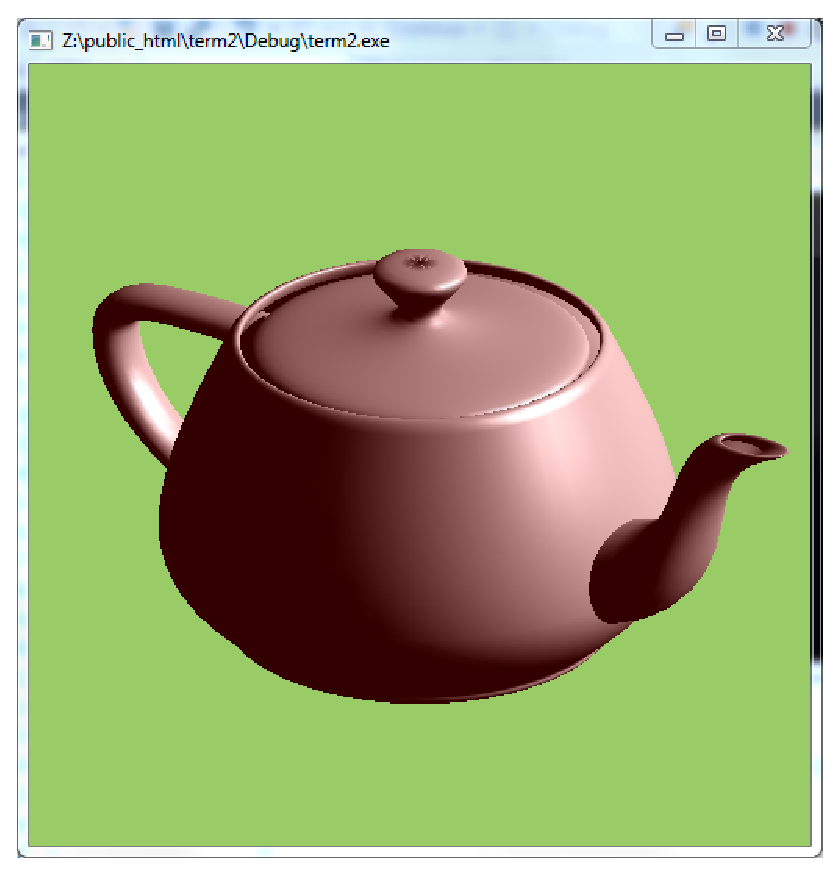
\includegraphics[width=1.75in]{termpicture/original.eps}
    &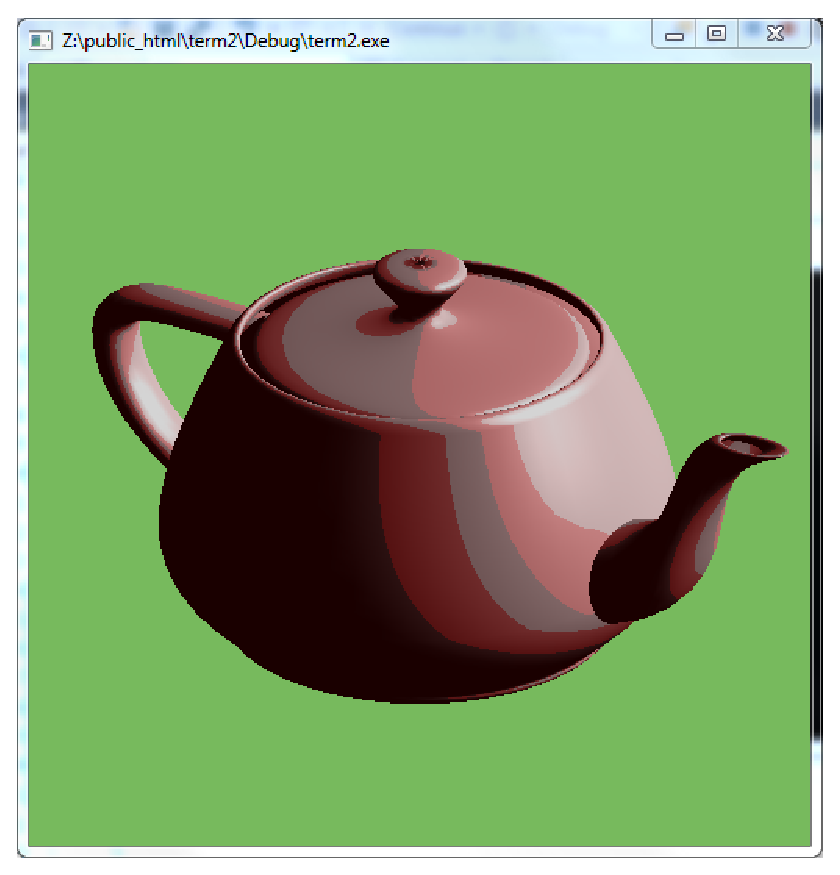
\includegraphics[width=1.75in]{termpicture/3valuesset.eps}
    &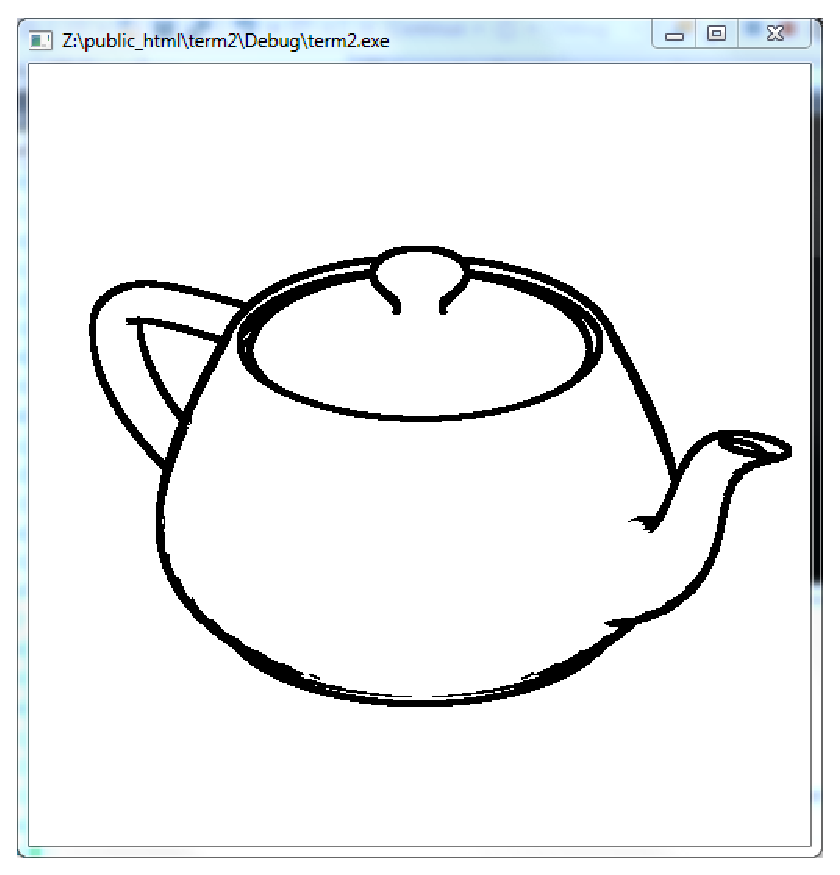
\includegraphics[width=1.75in]{termpicture/outlinesil0008.eps}
    &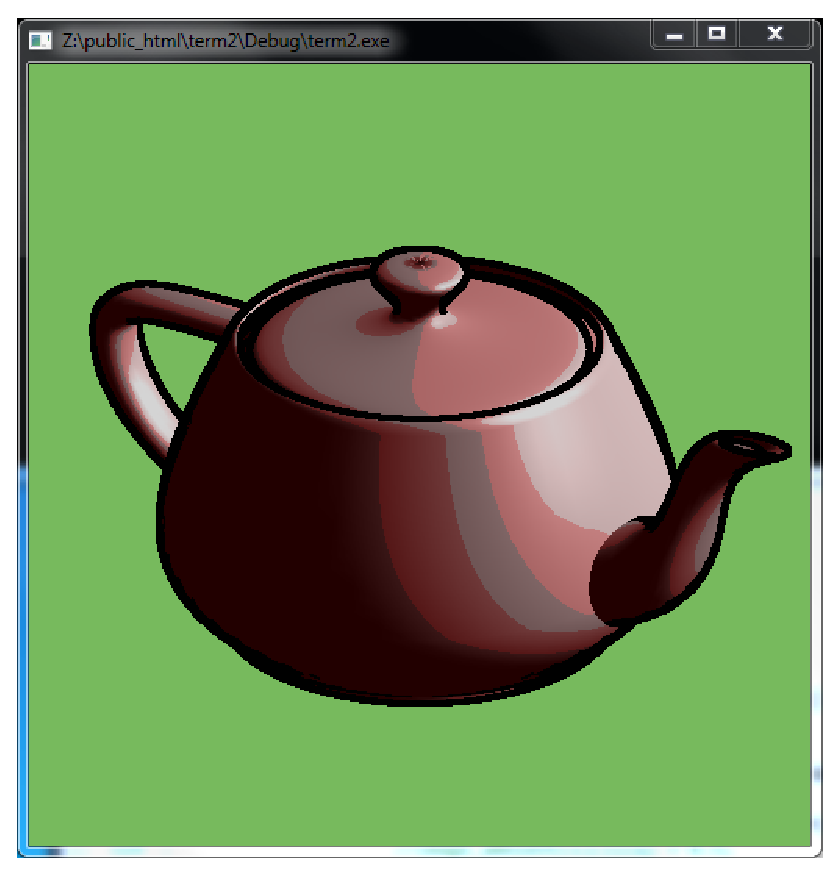
\includegraphics[width=1.75in]{termpicture/3valueoutline.eps}\\
    (a)   &  (b)  & (c)  & (d)
    \end{array}$
\caption{General rendering steps of cartoon-looking implementation: (a) the original rendering of a teapot, (b)
change the color into several uniformly colored areas, (c) the calculated outline of the teapot, and (d) combines (b) and (c) will result in a cartoon-looking-like image. Notice that the final picture (d) showed here are only a cartoon-looking-like image but not the final result of the implementation. } \label{fig:teapot} }

%% The ``\maketitle'' command must be the first command after the
%% ``\begin{document}'' command. It prepares and prints the title block.

\maketitle

%% Abstract section.

\begin{abstract}

\copyrightspace

The two biggest differences between {\em cartoon-looking} and {\em photo-realism} is that cartoon-looking image has constant size of outlines and uniformly colored areas. The algorithm introduced in this report is from  \cite{Decaudin:1996:CLR}, it not only covers these two main parts, but also bring in the texture, specular highlight, and shadow into the image. 

However, the implementation of this algorithm is quite complicated to achieve, so another version of the implementation is introduced and can also provide a {\em cartoon-looking-like} image. This kind of implementation is easy to implement and also has kind of specular light information and shadows. As for the result of outline-getting step, this algorithm also can provide a {\em sketch-like} image which contains some of the outline information.

\end{abstract}

%% ACM Computing Review (CR) categories.
%% See <http://www.acm.org/class/1998/> for details.
%% The ``\CRcat'' command takes four arguments.

\begin{CRcatlist}
  \CRcat{I.3.4}{Computer Graphics}{Paint systems};
\end{CRcatlist}

%% The ``\keywordlist'' command prints out the keywords.
\keywordlist


\section{Introduction}
\label{sec:intro}


%% The ``\copyrightspace'' command must be the first command after the
%% start of the first section of the body of your paper. It ensures the
%% copyright space is left at the bottom of the first column on the first
%% page of your paper.


In many conditions, people who studying computer graphics are intending to make the 3D-scenes more and more realistic. By doing the raytracing, rendering, calculating the reflections and shadows, the images we create today are closer and closer to the realistic objects. However, there are some other situations that people might need to have some cartoon-looking images. For example, creating the a 3D animation. Creating an animation by drawing every frame is really the past tense. This classic way of creating an animation not only requires a lot of work but also costs a lot of time and money. 

Based on the situation described above, developing an algorithm which can rendering every frame automatically is surely meaningful. The algorithm has been provided for a really long time, \cite{Decaudin:1996:CLR} talks about the algorithm which takes a 3D scene description as input and can automatically calculate the images. The image calculated by this algorithm contains not only the constant size of outlines and uniformly colored area, but also has textures, specular highlight, and shadow information. Texture is not necessary, but it will enrich and bring more details into the image. Specular highlight will provide a visual feedback of the material type of the objects. Shadows will provide the information that help to perceive the 3D aspect of the scene \cite{Decaudin:1996:CLR}. The shadow that this algorithm provide will result in two different colors on the object. The parts of the object in the shadow will have a darker color while the other parts are brighter. The edge between these parts are sharp, but not as soft as most of the situation we have in pooh-realism images.

The implementation this report provides is basically based on the algorithm mentioned above, but they will not be a hundred percent similar. The implementation this report uses is much easier to manipulate and can also result in a fairly good image. The shadows will be implement, and some of the light information will be kept, and also it will provide different types of the outlines for user to choose. Simply by setting some variable values can give the users different result of outlines, some of them are simpler while some of them have more details and can be treat as sketch images.

%%\begin{figure*}[t]
%%\begin{center}
%%    $\begin{array}{@{\hspace{-0.00in}}c@{\hspace{0.05in}}c@{\hspace{0.05in}}c@{\hspace{0.05in}}c@{\hspace{0.05in}}c}
%%    \includegraphics[height=1.3in]{images/tetra.eps}
%%    &\includegraphics[height=1.3in]{images/octa.eps}
%%   &\includegraphics[height=1.3in]{images/cube.eps}
%%    &\includegraphics[height=1.3in]{images/icos.eps}
%%    &\includegraphics[height=1.3in]{images/dodec.eps}\\
%%   \end{array}$
%%\end{center}
%%\caption{$N$-way rotational symmetries appear naturally in the
%%Platonic solids: tetrahedron ($N=2$), octahedron ($N=3$), cube
%%($N=4$), icosahedron ($N=6$), and dodecahedron ($N=10$). }
%%\label{fig:symmetry_examples}
%%\end{figure*}

\section{Algorithm}
\label{sec:algorithm}
The algorithm provided by the \cite{Decaudin:1996:CLR} is kind of complicated, but since this algorithm is the fundamental of this reports implementation, it will be fully described and explained in this report. Figure \ref{fig:workflow} shows the working flow of the whole algorithm, and it mainly can be divided into two parts: outlines and shadows. The outlines includes two parts which are silhouettes and crease edges. The shadows can be decided into two parts and they are backface shadows and projected shadows.
\begin{figure}[t]
\begin{center}
    $\begin{array}{@{\hspace{-0.00in}}c@{\hspace{0.05in}}c}
    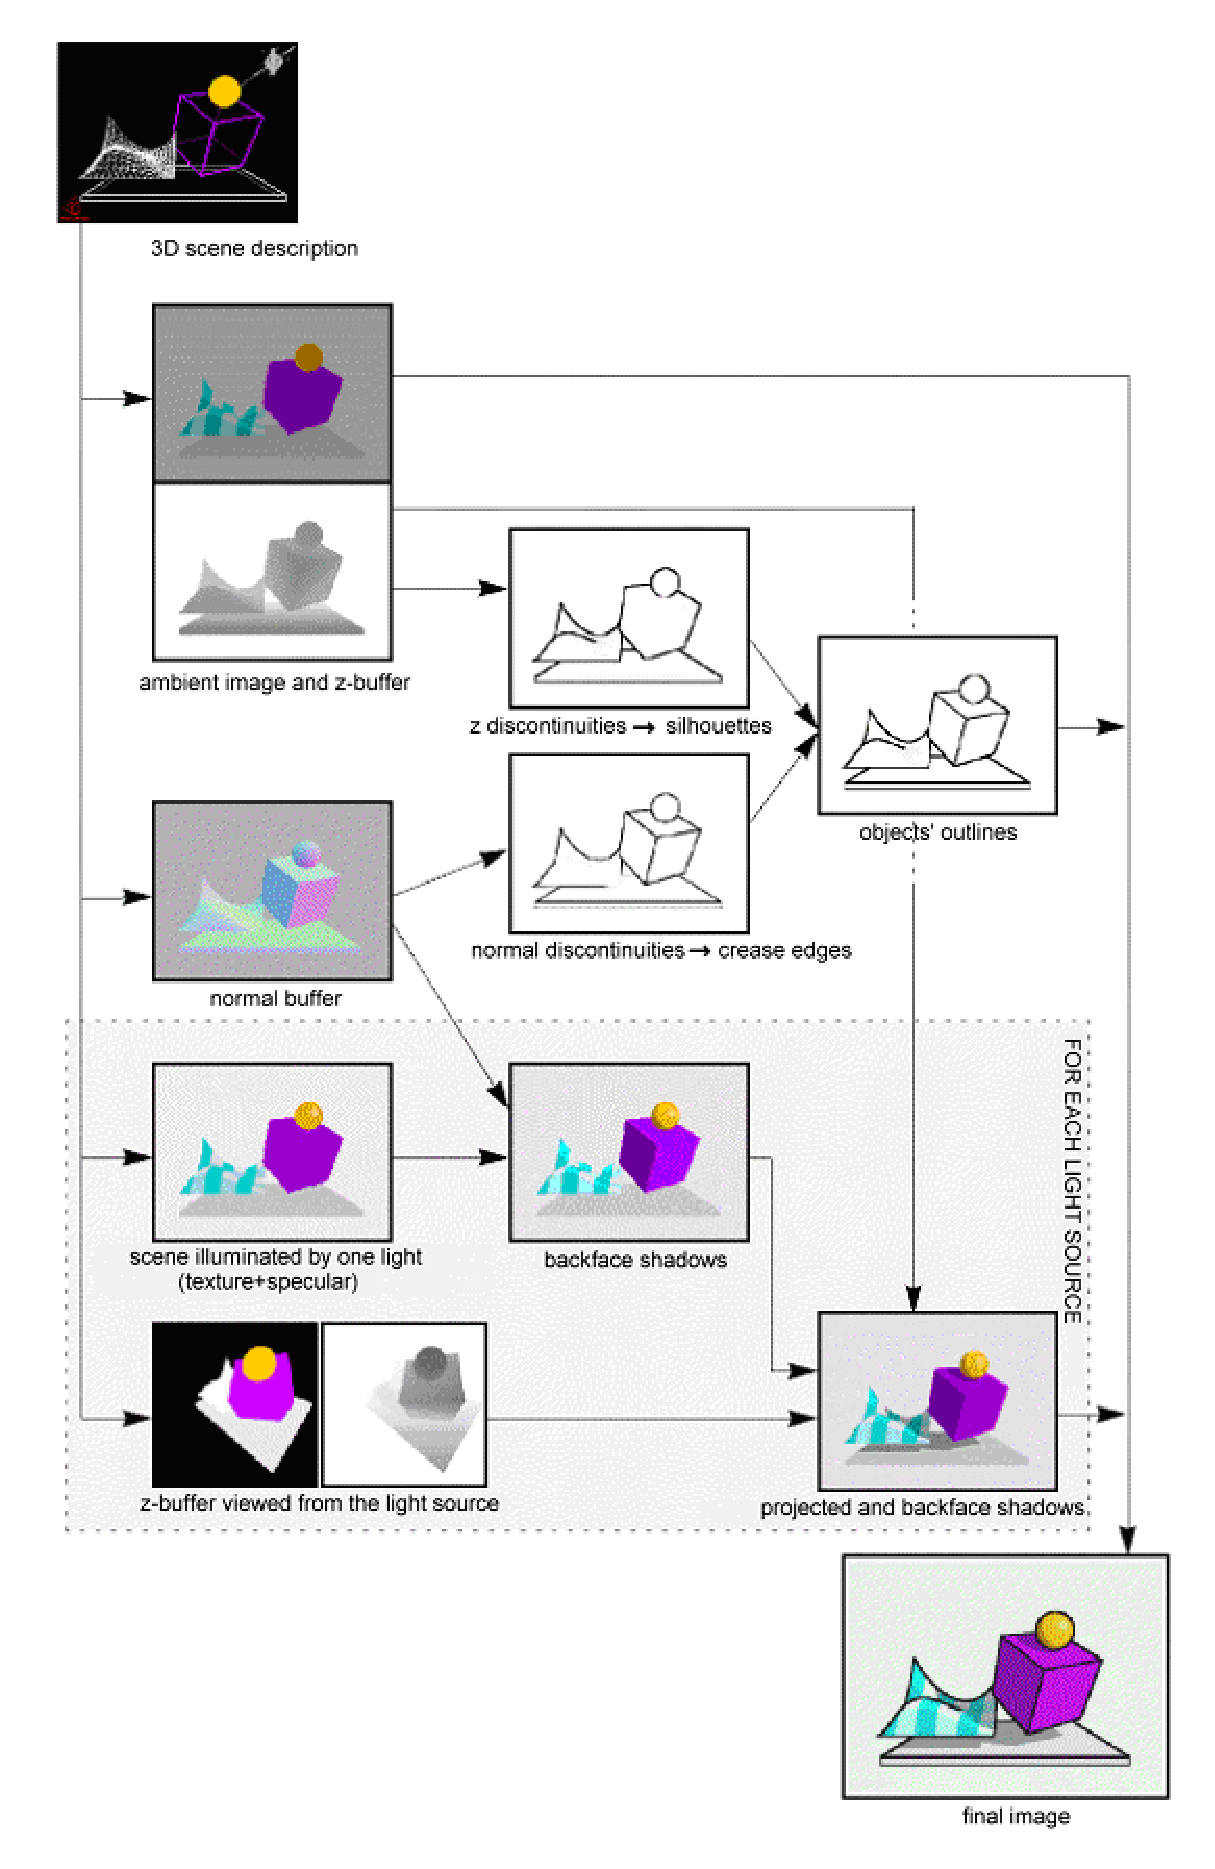
\includegraphics[width=3.5in]{termpicture/workflow.eps}
    \\
    \end{array}$
\end{center}
\caption{ The working flow of the algorithm, The part above creates the outlines and the part in the broken lines box creates the shadows. } \label{fig:workflow}
\end{figure}
First of all, the algorithm takes a 3D scene description as the input, and then it will render it with only ambient light on. This operation will result in a general form of the object which stands for the what it will be looked like from the camera position. The color filled in the form is constant and it will be treated as a par to the main color in the final cartoon-looking result. Just as  Figure \ref{fig:ambient} shows, it is the result that a teapot be rendered only with ambient light on. However, it need to be mentioned that this image not only stores the information as it shows up. This image will also stores the depth information even it looked not has depth at all. The depth information is a really important information that need to be used in the after steps. It will be fully described in the following sections. The printed out depth information is also showed in the Figure \ref{fig:ambient}.
\begin{figure}[t]
\begin{center}
    $\begin{array}{@{\hspace{-0.00in}}c@{\hspace{0.05in}}c}
    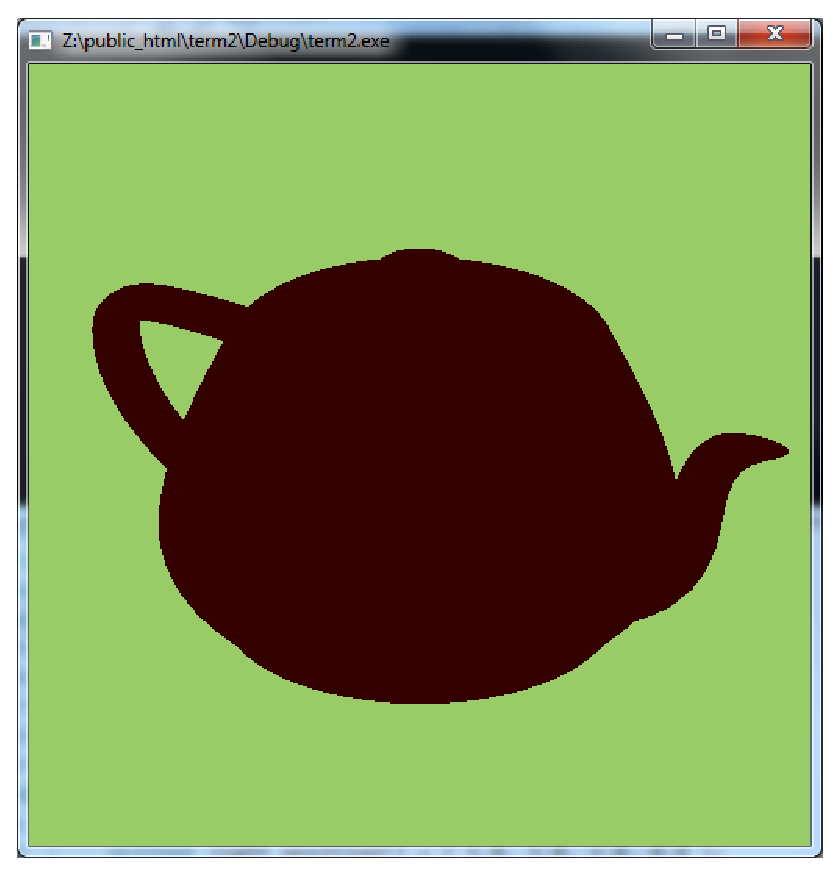
\includegraphics[height=1.5in]{termpicture/ambientonly.eps}
    &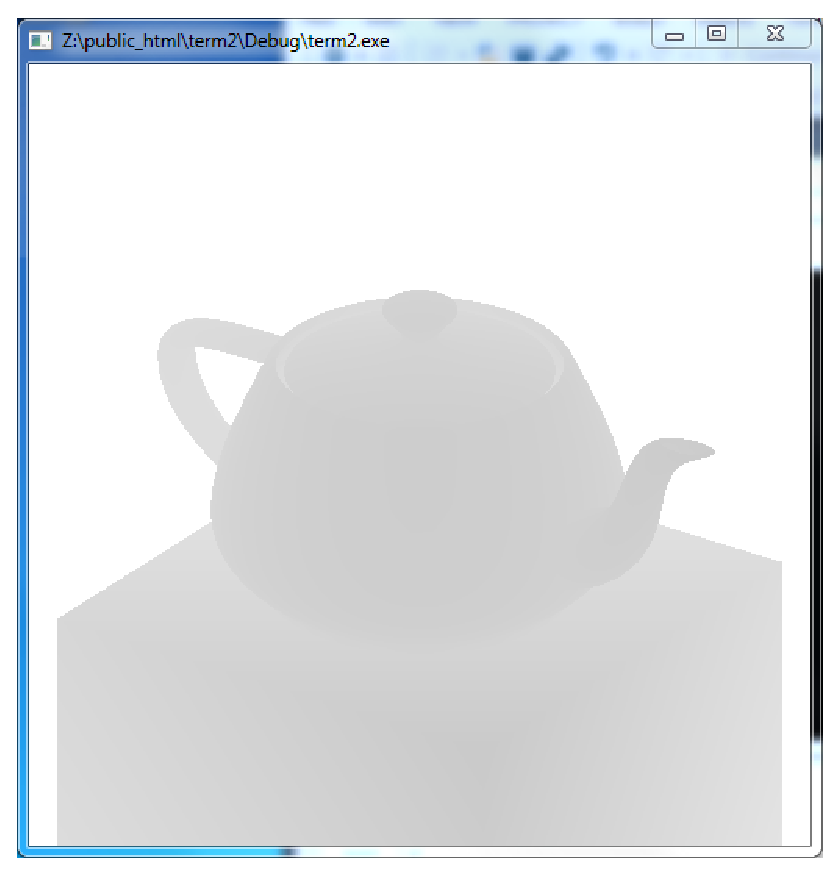
\includegraphics[height=1.5in]{termpicture/camerazbuffer.eps}
    \\
    (a) & (b)
    \end{array}$
\end{center}
\caption{ (a) rendering the teapot with only ambient light on, (b) printing out the z-buffer value from the camera original position. } \label{fig:ambient}
\end{figure}
\subsection{Outlines}
\label{sec:outline}
The outlines created in this algorithm can be decided into two different types. The one is silhouettes and another one is crease edges. Silhouettes correspond to places where the view direction is tangent to the object's surface \cite{Decaudin:1996:CLR}. Visible crease edges is always in the general outline of the object, in the image, it is usually in the middle of the objects, which gives the details about the edges that can be seen due to the view point.

The methods this algorithm uses to create the silhouettes and crease edges are quite similar, so the method creating silhouettes will be clearly explained, and about the method creating crease edges, this report will only introduce the differences.

The method creating silhouettes can be divided into two parts. The gradience of the z-buffer value will be calculated first, and based on the result we have, we will use a {\em non-linear filter} to determine where the outlines should be drawn. The way we use to calculate the z-buffer value gradience is using a counter direction filter on the pixel we choose and the eight neighbor-pixels around it. The equation listed below shows the way calculating the gradience of the z-buffer value. It should be noted that A, B and C are the three pixels in the pixel x, which is the chosen pixel, above line. D and E are the two pixels beside the pixel x. The F, G and H pixel are the pixels next to x in the next line. The reason why B, D, E, and G pixel are taken into count as double value is because they are the pixels direct connect to the pixel x. 
\begin{equation}
g=\frac{1}{8}(|A-x|+2|B-x|+|C-x|+2|D-x|+2|E-x|+|F-x|+2|G-x|+|H-x|)
\end{equation}
By calculating the gradience of every pixel, we can have a matrix which has the same size of the image, and every pixel position stores the z-buffer value gradience relate to that pixel. Then, the next step is to calculating the {\em edge-limit-value}, and compare it with every gradience we have in the pixel position. The way we create the {\em edge-limit-value} is by calculating the neighbors of that pixel position again using a {\em non-linear filter}. The equation showed blow is the way that algorithm uses to calculate the {\em edge-limit-value}. It should be noted that the $g_max$ and $g_min$ in the equation come from the gradience values around the selected pixel x and its eight neighbors. 
\begin{equation}
p=min\{ (\frac{g_max - g_min}{k_p})^2, 1 \} \label{eq:calq}
\end{equation}
The $k_p$ showed in the above equation is the detection threshold in-between 0 and 1. The lower $k_p$ is the more silhouettes will be detected \cite{Decaudin:1996:CLR}. The difference of the outlines we get by using different $k_p$ value will be introduced in the implementation part.
\begin{figure}[t]
\begin{center}
    $\begin{array}{@{\hspace{-0.00in}}c@{\hspace{0.05in}}c}
    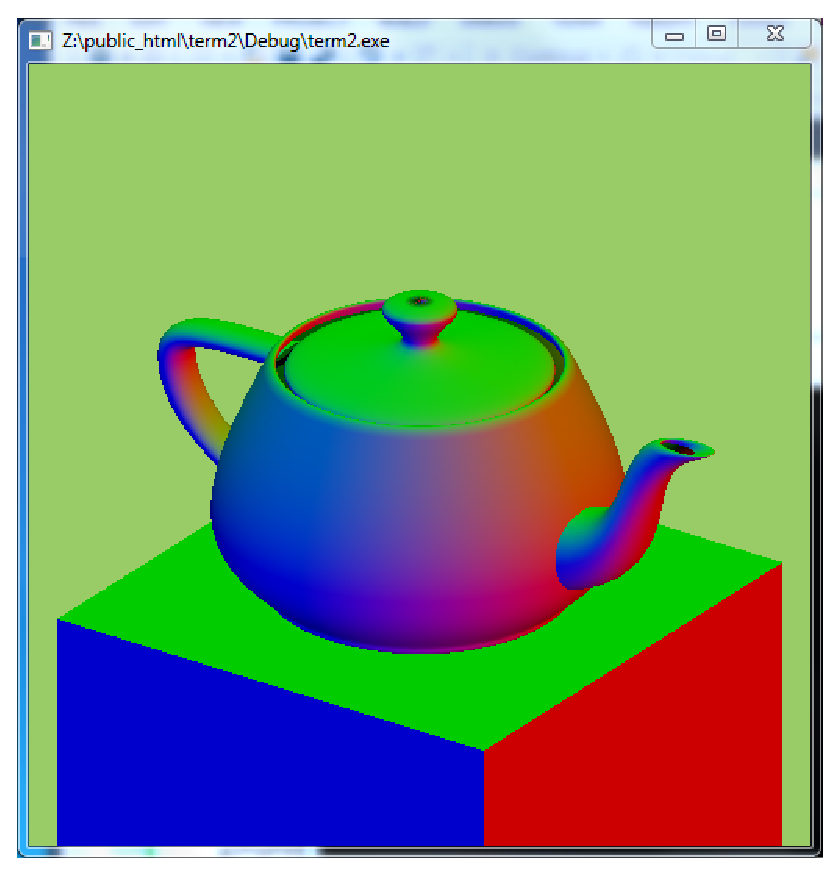
\includegraphics[height=1.5in]{termpicture/normalI1.eps}
    &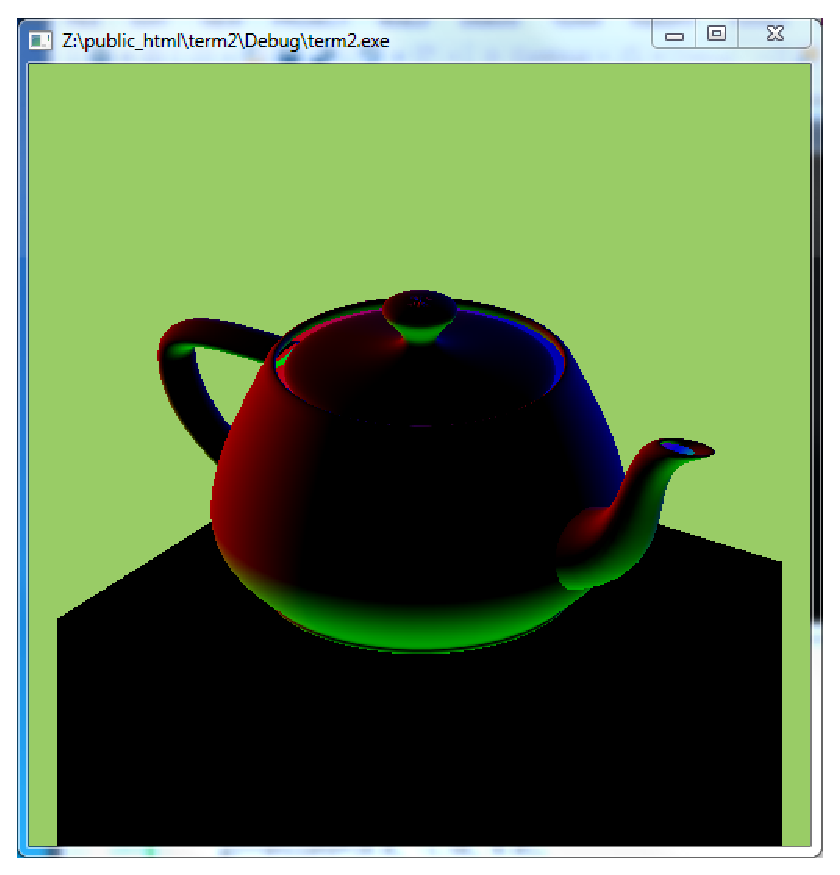
\includegraphics[height=1.5in]{termpicture/normalI2.eps}
    \\
    (a) & (b)
    \end{array}$
\end{center}
\caption{ (a) $I_1$ image with red light at +x direction, green light at +y direction, and blue light at +z direction, (b) $I_2$ image with red light at -x direction, green light at -y direction, and blue light at -z direction. } \label{fig:normal}
\end{figure}
By following the steps mentioned above the algorithm will provide a silhouettes, as for the crease edges, we will use the same type of calculation mentioned above. However, the differences between these two types of outline is that the equations will be used on different buffers and the $k_p$ value will be set in different ways. The buffer that will be calculated with is no longer the z-buffer we used above, it will be that {\em normal buffer}. The way to create a normal buffer is that we will render two more images first, each image will has three light sources on. As the Figure \ref{fig:normal} shows above, for the first rendered image $I_1$, the three lights will be a red light at +x direction, a green light at +y direction, and a blue light at +z direction, the second rendered image $I_2$ will have three lights which are red light at -x direction, green light at -y direction, and blue light at -z direction. We will render these two images with the color calculated based on the two equations showed below. Then in order to get the final normal buffer, we will subtracting these two renderings $I_1 - I_2$ to get a buffer in which each component red, blue, green corresponds to $n_x$, $n_y$, $n_z$ respectively. It also should be mentioned that the $n_x$, $n_y$, $n_z$ mentioned above and shown in the equation is the three coordinates of the normal associated to the corresponding 3D point \cite{Decaudin:1996:CLR}.
\begin{equation}
color= red * max\{n_x, 0\} + green * max\{n_y, 0\} + blue * max\{n_z, 0\}
\end{equation}
\begin{equation}
color= red * max\{-n_x, 0\} + green * max\{-n_y, 0\} + blue * max\{-n_z, 0\}
\end{equation}
By using the same calculation on the z-buffer mentioned above on the normal buffer we just calculated, the result will shows up as the crease edges we want. Finally, by simply combine these two types of outlines, the algorithm will provide the final version of outlines as the result.
\subsection{Shadows}
\label{sec:shadow}
In order to implement shadows, we will use only one light source a time due to the situation that multiple light sources might be added into the 3D description. Two types of shadows will be calculated in this algorithm, one is backface shadows and another one is projected shadows. However, before calculating the shadows, we need to render the image first. 

The basic idea to rendering the image is to remove the {\em dot product} of the object's normal and the light vector from the {/em Phong shading equation}. If the object is specular, then the specular highlight will be kept because it provides information about object's material type \cite{Decaudin:1996:CLR}. In order to achieve the goal, the algorithm will first copy the diffuse color into ambient, then set the diffuse color to black, and also keep the specular. By doing in this way, it will result in an image where each object is uniformly colored by its diffuse color. Also by doing this, the texture and the specular highlight information will be stored in the image.

in order to create the backfire shadows, the algorithm will just simply examine the {\em dot product} of the selected point's normal and the its light vector. Because of the fact that the backface shadows are just the object areas opposed to the light source \cite{Decaudin:1996:CLR}, if the dot product results in a negative value, then the selected point is in the shadow and its color needs to be darken.
\begin{figure}[t]
\begin{center}
    $\begin{array}{@{\hspace{-0.00in}}c@{\hspace{0.05in}}c}
    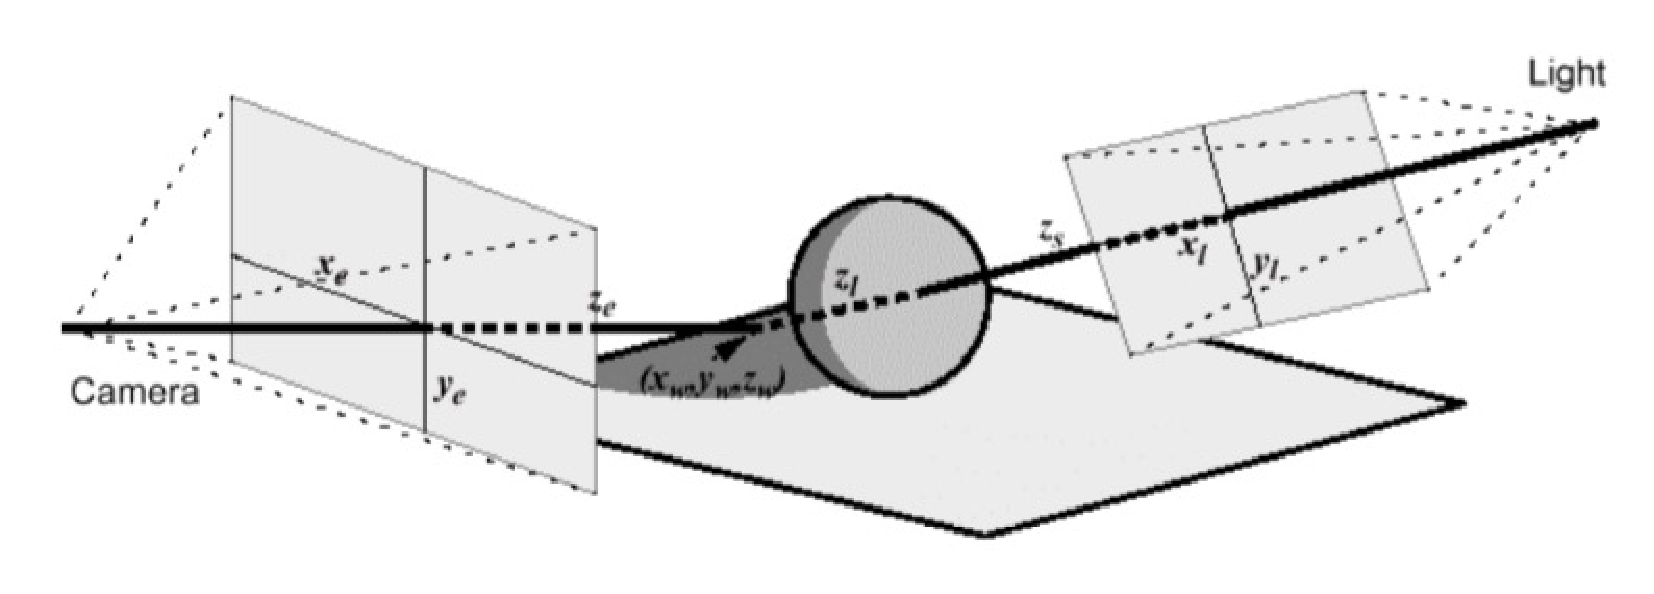
\includegraphics[width=3.5in]{termpicture/shadowmap.eps}
    \\
    \end{array}$
\end{center}
\caption{ The shadow map technique used to calculate projected shadows. } \label{fig:shadowmap}
\end{figure}
Calculating the projected shadows is more complicated than implementing backface shadows, the algorithm uses a technique named "shadow map". As the Figure \ref{fig:shadowmap} shows above, this technique can be divided into several steps. The first step is to calculate every pixie's coordinate in the image rendered from camera position int the real 3D world coordinate. The pixel coordinate $(x_e, y_e, z_e)$ is relate to the position this pixel in the image pixel matrix, the $z_e$ value is from the z-buffer value in this camera position. The calculated world coordinate $(x_w, y_w, z_w)$ will be taken into next step's calculation. Then we will set the camera to the lighted light position, and rendering the image again in order to get the z-buffer value from the new camera position. The world coordinate $(x_w, y_w, z_w)$ will be calculated into a new pixel coordinate in the image rendered from the light position, and they will be stored in to $(x_l, y_l, z_l)$. By comparing the new $z_l$ value from the new image with the new z-buffer value of the point $z_s$, the algorithm will determine whether the point is in the shadow or not. If $z_l < z_s$, then the point is not "seen " by the light, in another words, it is in the shadow. Except this kind of condition, then the point will be lighted up. 

By combining these two types of shadows with the image rendered at the beginning of the shadow step, we will get a image with detailed texture and specular highlight information alone with both backface shadows and projected shadows.
\subsection{Final result}
\label{sec:final}
To create the final result, the algorithm will take the advantage of the previous image rendered with only ambient light on, the final result of outline calculating, and the final result of the shadow rendering. By using the equation mentioned below, the algorithm will provide the final cartoon-looking image. It should be mentioned that the reason why it uses outline in $(1 - outline)$ way is because outlines are just black pixels, so we want those pixels in the outline area be colored into black. In order to do this, we will set the original outline pixels' value 1 into 0, and set other pixels' value from 0 back to 1.
\begin{equation}
image = (ambient image + several shadows' result) * (1 - outlines)
\end{equation}
\section{Implementation}
\label{sec:implementation}
The algorithm from \cite{Decaudin:1996:CLR} has been fully explained in the previous section. However, the whole algorithm is quite complicated and not easy to implement. The method this report using to implement the cartoon-looking image is easier to understand and implement. This method also covers the content size outline, the uniformly colored area, and the shadow. As the extra result of implementing outlines, the method to create a sketch-looking outline is also introduced in the following sections. The implementation will mainly be introduced in three parts, and they are color, outline and shadow. As showed in the Figure \ref{fig:original2}, the example image used in this section is more complicated than a simple teapot used in previous section. In order to show the shadows, a cube is added at the bottom of the teapot.
\begin{figure}[t]
\begin{center}
    $\begin{array}{@{\hspace{-0.00in}}c}
    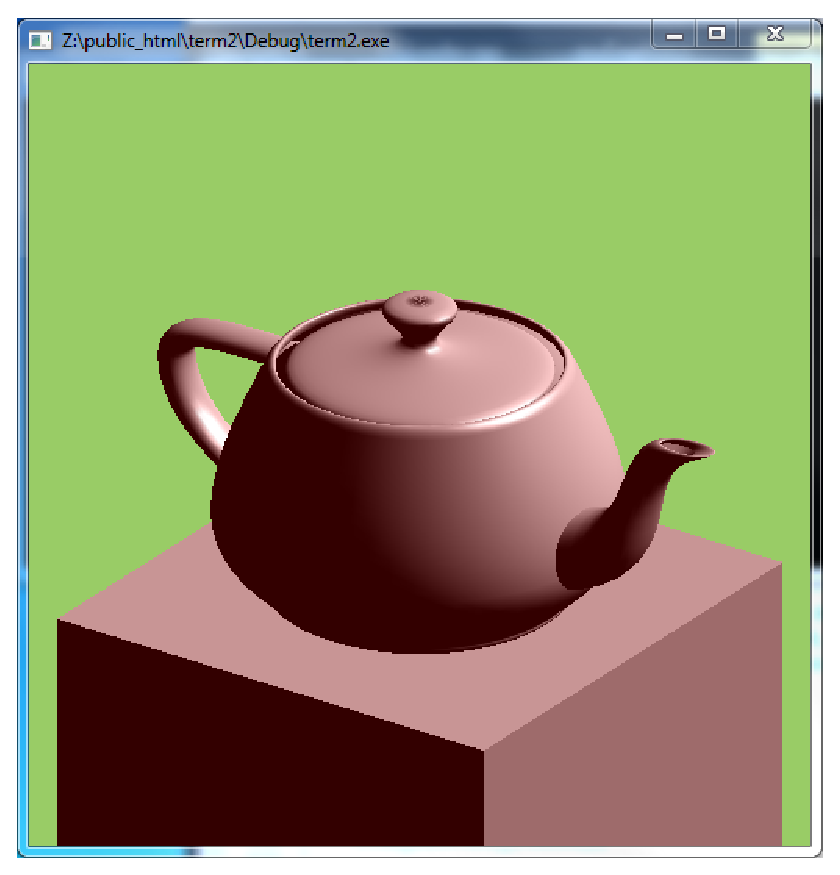
\includegraphics[height=2.15in]{termpicture/original2.eps}
    \\
    \end{array}$
\end{center}
\caption{ The original image used to show the implementation result. } \label{fig:original2}
\end{figure}
\subsection{Color}
\label{sec:colorimp}
In the original algorithm, the color comes from the image only rendered with ambient light on and the images rendered with only one light source on. The after one also provides the texture and specular light information. However, rendering the images with every light source on could be a pain in the neck. To implement these pictures, we need to change the setting of the light several times (number of light source times) and render one image every time. Also, to render these images, we should doing a lot other operations, for example copying the diffuse color into ambient and keeping the specular light information. 

The method this report using is far easier than the original method. By using only a few lines of code, the OpenGL will render the 3D description into a normal photo-realism image. By manipulating the existing photo-realism image, setting a range of the value of RGB colors, we will have the result that the object be filled up with several uniformly color area, just like (b) image in the Figure \ref{fig:teapot}. To implement the uniformly colored area, this report is using the method to separate the range of RGB color into three parts, which is from 0 to 0.33, 0.34 to 0.66, and 0.67 to 1 in the normalized condition. By setting the pixel color information in the different range with different constant value plus its original value divided by a constant number, we will result in several uniformly colored area. The detailed equation is showed below.
\begin{equation}
color= \left\{ \begin{array}{ll} color / 1.5 & \textrm{ if $color < 0.33$} \\
 0.33 + (color - 0.33) / 2 & \textrm{ if $0.34 \le color < 0.66$}
\\ 0.66 + (color - 0.66)/2 & \textrm{ if $0.67 \le color$} 
\end{array} \right.  \label{eq:color_set}
\end{equation}.
\subsection{Outline}
\label{sec:outlineimp}

In the original algorithm, the outline is divided into two different types, the silhouette and the crease edge. However, implementing crease edges requires the normal buffer calculating. To calculating the normal buffer we need to calculate the normal of every point related to every pixel in the image. This relates to a bunch of lines of code and also hard calculation formulas. To simplify the calculation and the implementation, a decision that give up calculating the normal buffer has been made in this report. So the method of calculating outlines used in implementation in this report is just doing the silhouette using the equations mentioned in the previous section. As the Figure \ref{fig:diffvalue} shows below, by setting different value of {\em edge-limit-value} and $k_p$ in equation \ref{eq:calq}, it also can achieve the crease edges, even though the teapot contains so many unnecessary outlines.
 \begin{figure}[t]
\begin{center}
    $\begin{array}{@{\hspace{-0.00in}}c@{\hspace{0.05in}}c}
    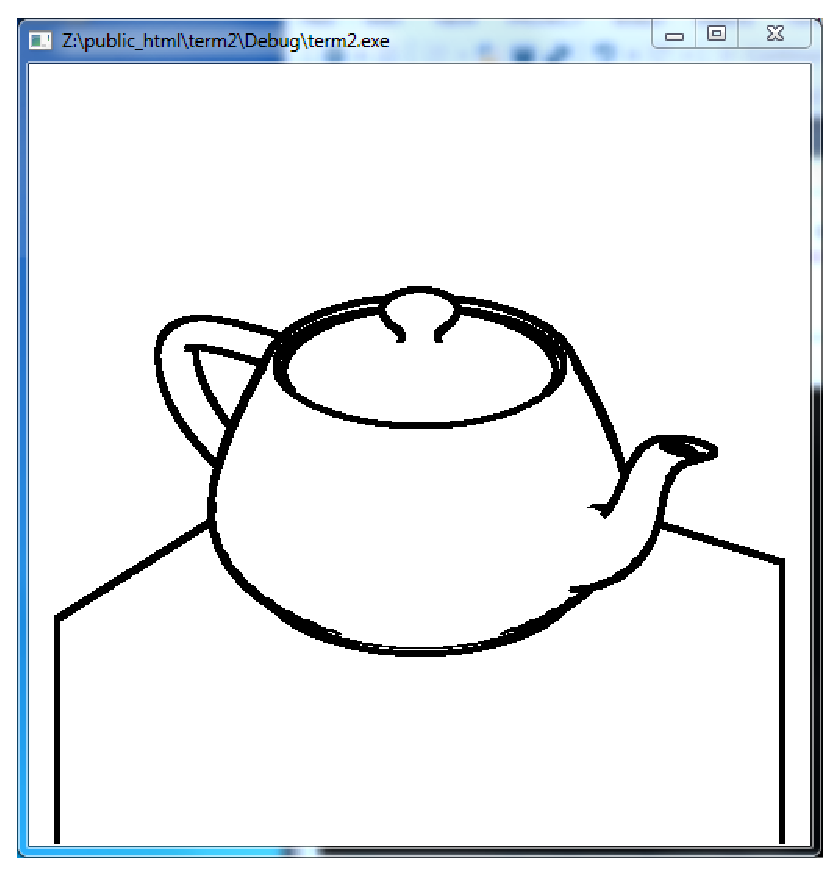
\includegraphics[height=1.5in]{termpicture/outlinesil000807.eps}
    &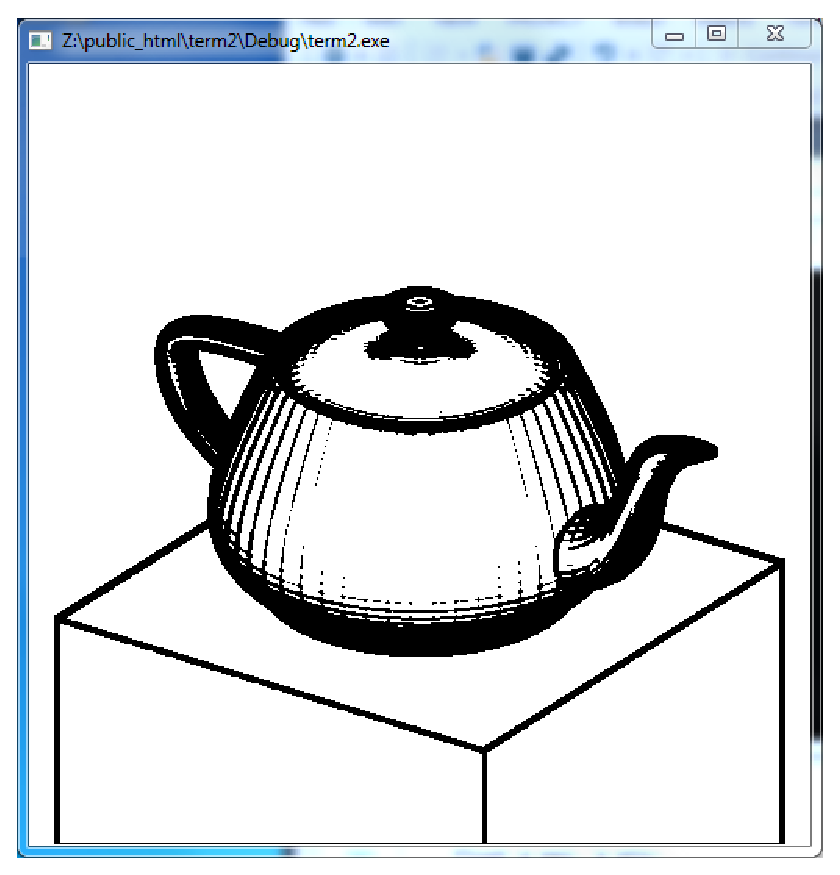
\includegraphics[height=1.5in]{termpicture/outlinesil000102.eps}
    \\
    (a) & (b)
    \end{array}$
\end{center}
\caption{ (a) set $k_p = 0.0008$ and {\em edge-limit-value} = 0.7, (b) set $k_p = 0.0001$ and {\em edge-limit-value} = 0.2. Note that the teapot in (b) contains some unnecessary outlines.} \label{fig:diffvalue}
\end{figure}
To rendering the cartoon-looking image, we only need a simple outline such as (a) in Figure \ref{fig:compke}. However, during the implementation, it is found that some outlines looked like sketch is also pretty. By comparing the images using different {\em edge-limit-value} and $k_p$ value in Figure \ref{fig:compke}, it is easy to find out that the lower $k_p$ is, the more silhouettes will be detected \cite{Decaudin:1996:CLR}. Also, the lower {\em edge-limit-value} is, the wider outline is. By setting suitable values of {\em edge-limit-value} and $k_p$, we can create the sketch image as we want. In the Figure \ref{fig:compke}, (b) is the best sketched teapot, and its {\em edge-limit-value} = 0.7 and $k_p = 0.00015$.
 \begin{figure}[t]
\begin{center}
    $\begin{array}{@{\hspace{-0.00in}}c@{\hspace{0.05in}}c@{\hspace{0.05in}}c}
    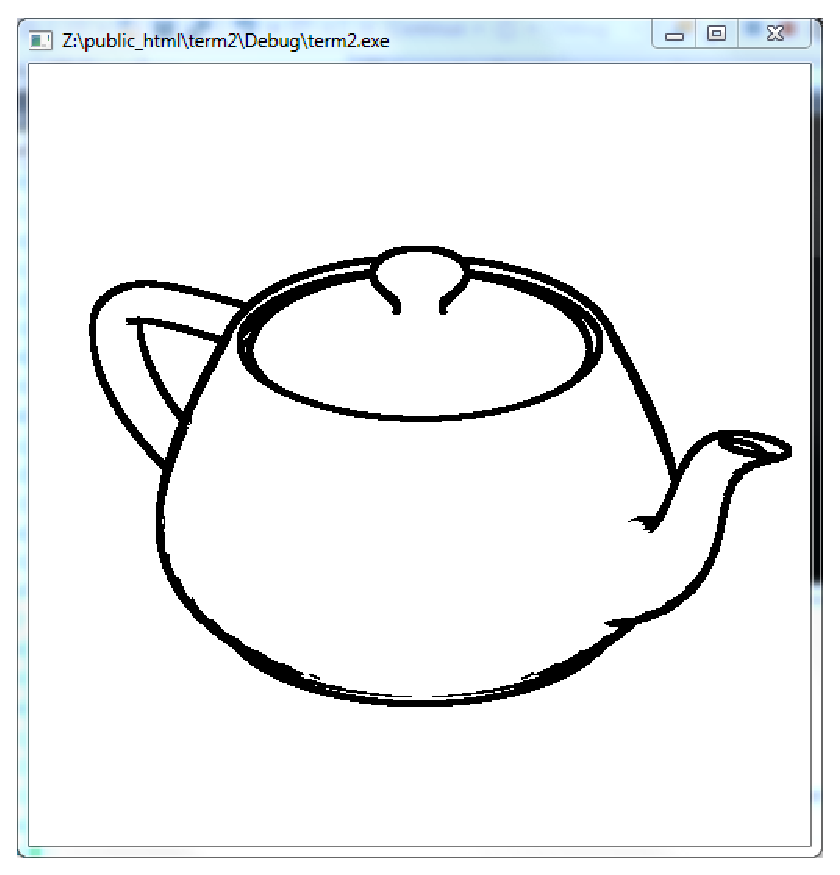
\includegraphics[height=1.1in]{termpicture/outlinesil0008.eps}
    &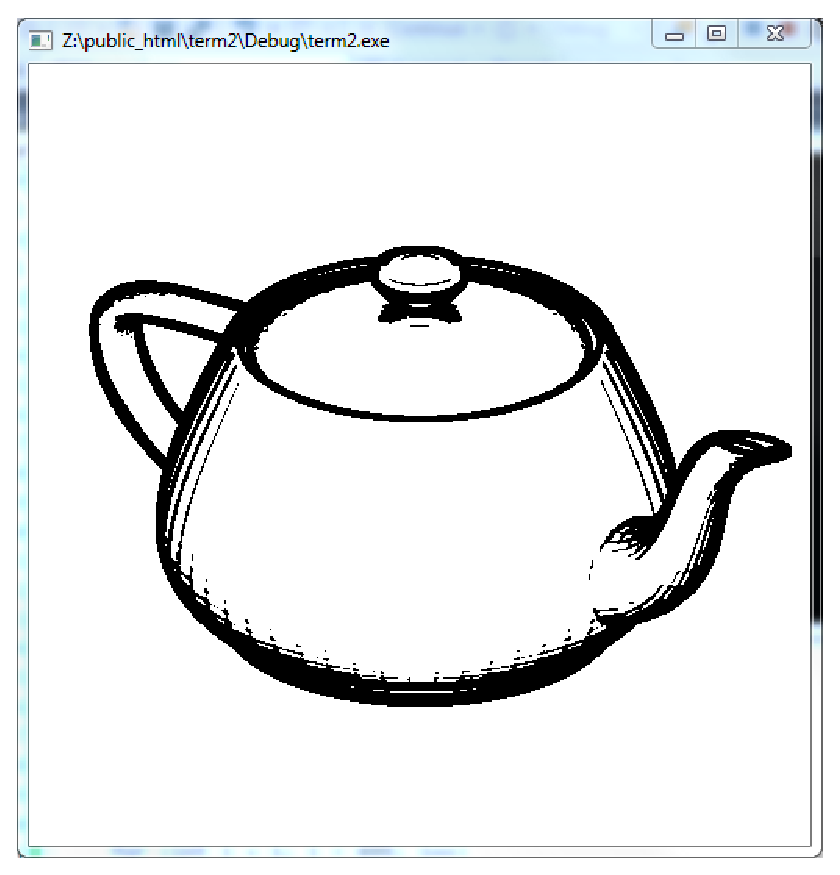
\includegraphics[height=1.1in]{termpicture/outlinesil0001507.eps}
    &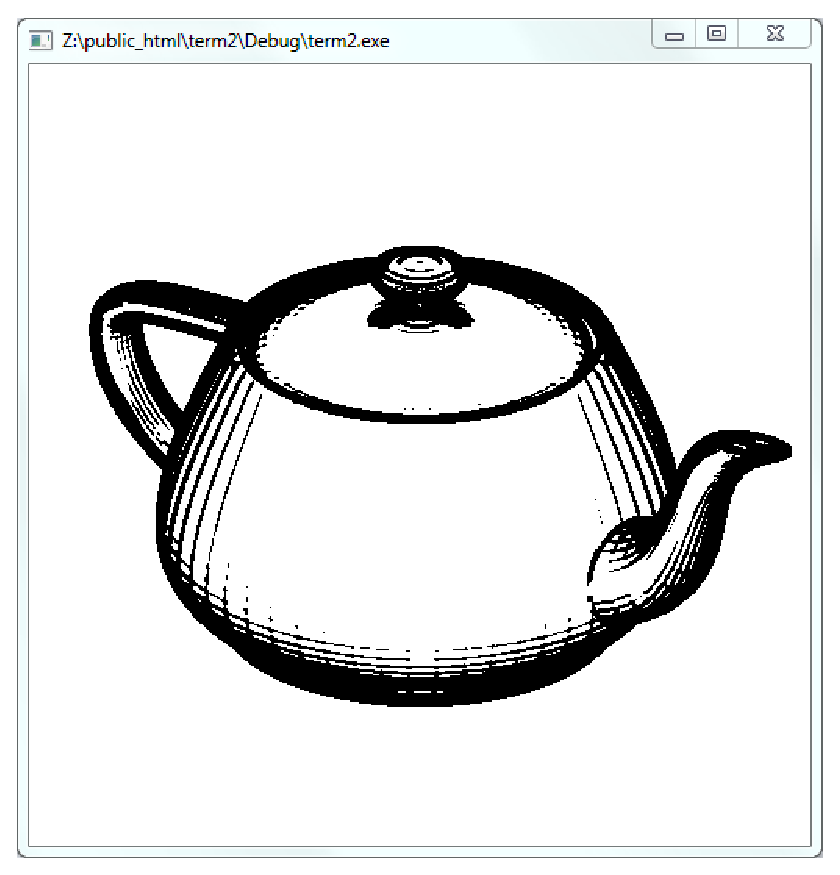
\includegraphics[height=1.1in]{termpicture/outlinesil0001502.eps}
    \\
    (a) & (b) & (c)
    \end{array}$
\end{center}
\caption{ (a) set $k_p = 0.0008$ and {\em edge-limit-value} = 0.7, (b) set $k_p = 0.00015$ and {\em edge-limit-value} = 0.7, (c) set $k_p = 0.00015$ and {\em edge-limit-value} = 0.2.} \label{fig:compke}
\end{figure}
\subsection{Shadow}
\label{sec:shadowimp}
The original algorithm introduced in this report covers two types of shadows. One type is backface shadows and another type is projected shadows. The reason why it includes two types of shadows is that the original algorithm's principle is to render a 3D cartoon using the 3D objects' description, and in the cartoon there two types of objects, one type is the constant constructions and another type is the moving objects. The backface shadows relates to the constant constructions which cannot move, and the projected shadows relates to the moving objects. Due to the principle of this report is to rendering the static objects, it is decided that cutting down one type of the shadows. Since in order to simplify the implementation, the normal buffer has already been given up in the outline calculation, and the backface shadows requires the calculating of it, it is decided that this report will only implement the projected shadows. 
 \begin{figure}[t]
\begin{center}
    $\begin{array}{@{\hspace{-0.00in}}c@{\hspace{0.05in}}c}
    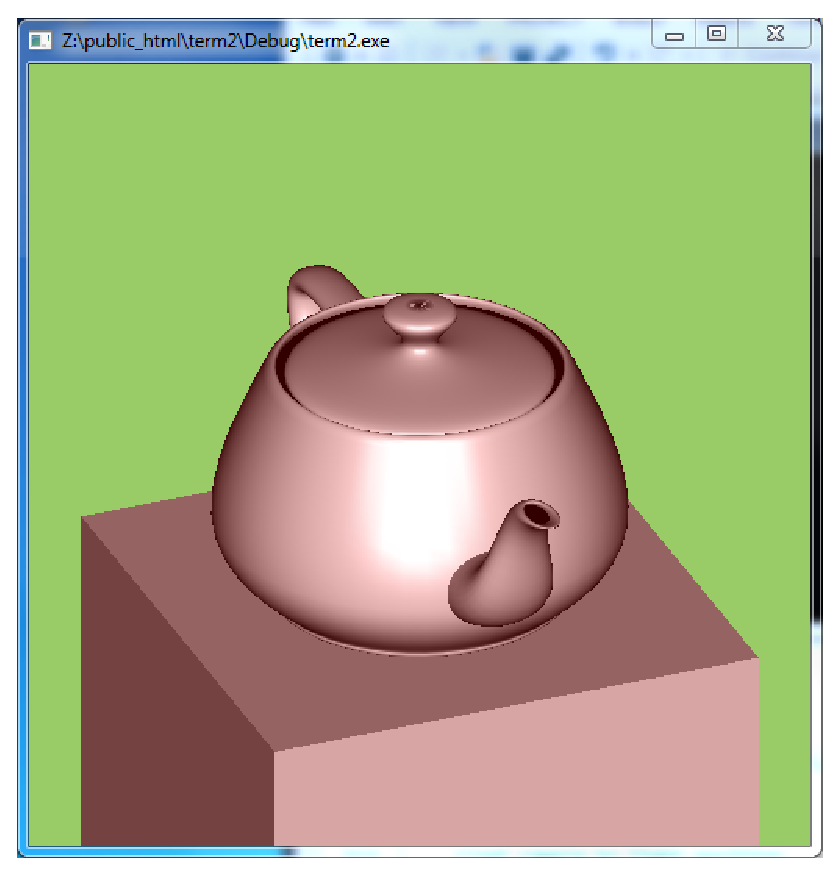
\includegraphics[height=1.5in]{termpicture/lightpos.eps}
    &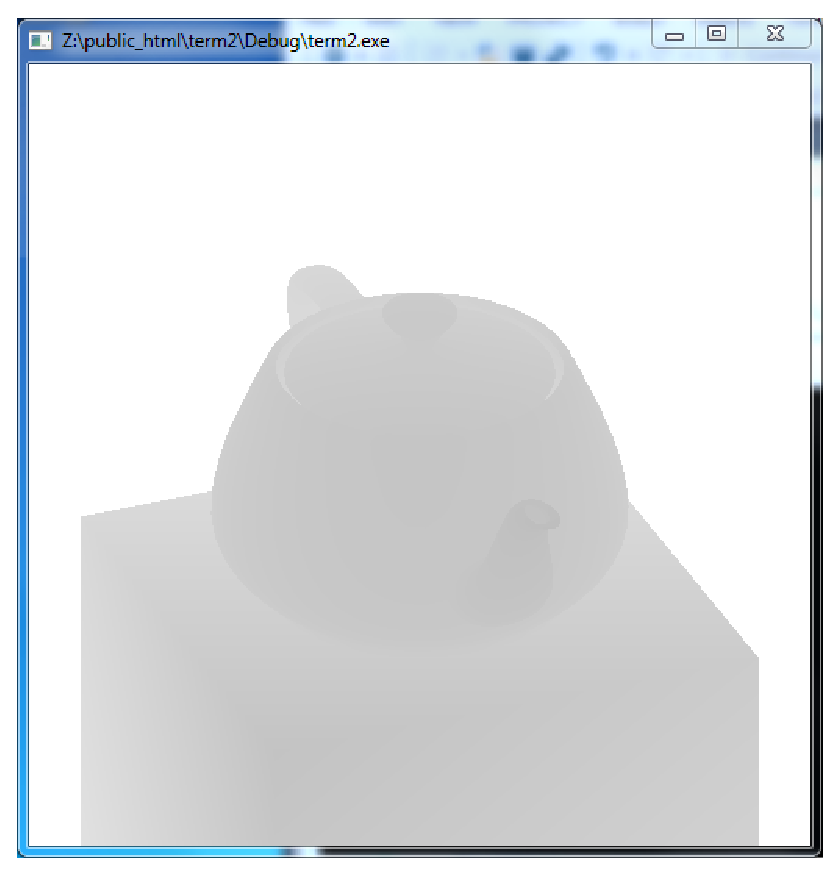
\includegraphics[height=1.5in]{termpicture/lightzbuffer.eps}
    \\
    (a) & (b)
    \end{array}$
\end{center}
\caption{ (a) the photo-realism rendering from the light position, (b) the z-buffer value from the light position.} \label{fig:lightpos}
\end{figure}

As it showed in the Figure \ref{fig:lightpos}, to calculate the projected shadows, the first step is to set the camera to the lighted up light position. By rendering a photo-realism image at that position, it is able to get the z-buffer value of the image. The following step is as similar as the original algorithm described in the previous section. The pixel coordinate in the image with the z-buffer value from the original camera position will be transformed into the 3D world coordinates. After changing the camera to the light position, every point in the 3D world coordinate which relate to the original image pixel will be transformed to the new image coordinate rendered from the light position. By comparing the coordinate z axes value to the z-buffer value we get in previous step, it is able to determine whether the pixel in the original image should be darken or not. If the z axes value is larger than the z-buffer value, then the point in the 3D world coordinate is in the shadow. In another word, the pixel in the original image relate to this point should be darken.
\begin{figure}[t]
\begin{center}
    $\begin{array}{@{\hspace{-0.00in}}c}
    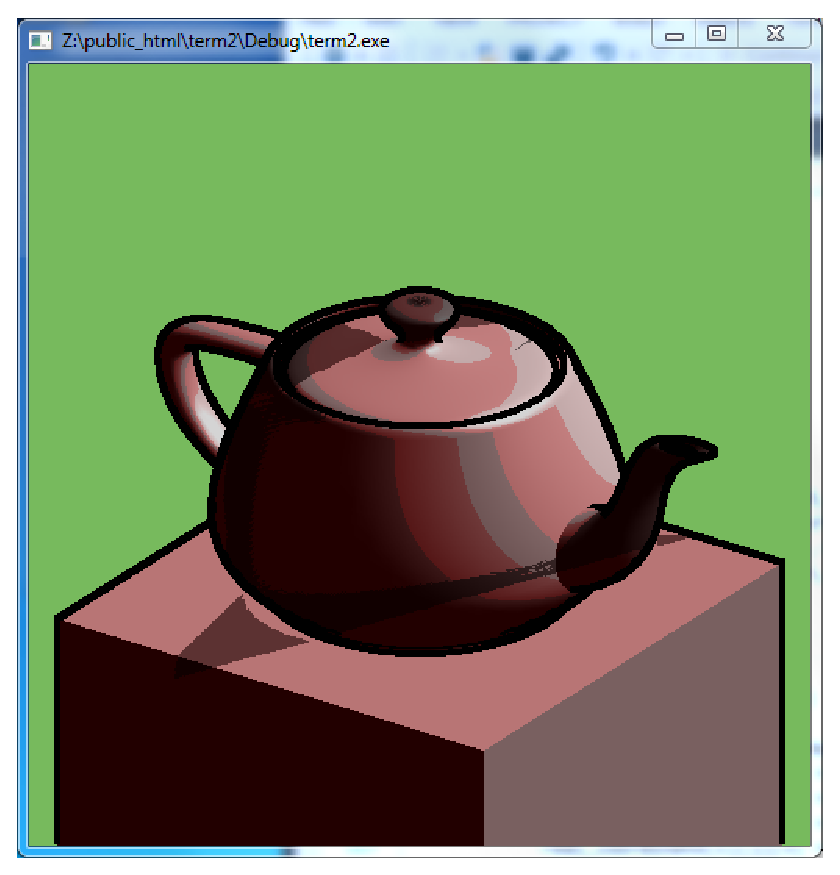
\includegraphics[height=2.15in]{termpicture/wrongshadow.eps}
    \\
    \end{array}$
\end{center}
\caption{ The last result of the implementation, the shadow exists but not in the right form. } \label{fig:wrong}
\end{figure}

However, as it shows in the Figure \ref{fig:wrong}, the final result this report has is not good enough to implement the right form of shadows. The problem is related to the coordinate transformation. By plotting the z axes value get from the final calculated result, it shows an image looked exactly like the z-buffer value image get from the original camera position. So it is obviously that the problem relies on the coordinates transformation part. The way this report use to do the coordinates transformation is by calling the OpenGl function "gluProject" and "gluUnproject". There might exist some wrong by calling these two functions.
\section{Conclusion}
\label{sec:conclusion}
This report mainly does two things. It introduces an algorithm published by Philippe Decaudin in 1996 \cite{Decaudin:1996:CLR}, which can render a 3D scene description into cartoon-like images. This report fully explains the algorithm and also comes up with an original implementation to do almost the same thing. The implementation introduced in this report is doing the similar thing as the original algorithm does, but it create the result in a easier way, which simplify the original algorithm. The implementation mentioned in this report not only render the cartoon-looking image with constant size outline, uniformly colored area, and shadows, but also provides a simple way to create a sketch-like outline which could be treated individually. The final result of the implementation is not  perfect. The shadow it draws is  still in a wrong form. However, it also mentions the reason why this problem happens, so some more further work is needed.
\section{Further work}
\label{sec:further}
The further work of this implementation is obviously. Correcting the projected shadow will be the first thing that needs to be fixed. There also exists some other jobs that could be added into this implementation. As the original algorithm shows, it is necessary for the rendering to handle both backface and projected shadows if it is used to render a 3D animation has both static and moving objects. Also, adding the normal buffer into the implementation will bring more details into the image, so it could also be done. The goal is not to completely follow the original algorithm but finding a more simple way to implement the cartoon-looking rendering.
\section*{Acknowledgements}

I would like to thank the friendly TA Wojtek Rajski. He shows really a lot patient to me to help me doing the implementation. This work cannot be done on time without his help. I would also like to thank the professor Eugene Zhang who is teaching this class, I have learned a lot from this class and my programming skill with OpenGL has been pushing increasing all the way along this term.

%\fontsize{8pt}{8pt}\selectfont
%\itemsep 0.0in
%\parskip 0.03in
%\parsep 2pt


\bibliographystyle{acmsiggraph}
\nocite{*}
\bibliography{cartoonr}
\end{document}
